% make sure not a repeat header!
\subsection{Getting started in EA}
\visHeader
\hypertarget{static:starting vis}{}

You can begin modeling Leitner's Box in one of two ways - you can build the diagrams in the same workspace as the Part I demo by
opening the old \texttt{`demo.eap'} file, or you can start afresh by going to ``New Metamodel Project,'' choosing to start a new visual project without a demo
(Fig.~\ref{fig:new_visModel}), and opening that \texttt{.eap} file. This handbook has assumed you prefer the latter, which is reflected in the screenshots.
If you use the previous files, please note that the steps are exactly the same, but our package explorers may not match exactly. Keep a sharp eye out for
footnotes which explain the few differences.

\begin{figure}[htbp]
	\centering
  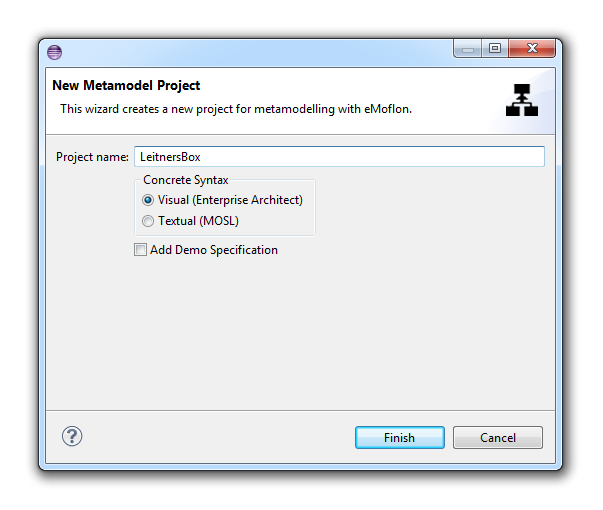
\includegraphics[width=0.7\textwidth]{eclipse_newMetamodelVisualPlain}
	\caption{Starting a new visual project}
	\label{fig:new_visModel}
\end{figure}

\newpage
\begin{itemize}
\item[$\blacktriangleright$] From EA, select your working set and click on the \texttt{Add a Package} button (Fig.~\ref{fig:new_package}).

\begin{figure}[htbp]
	\centering
  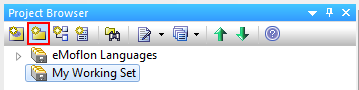
\includegraphics[width=0.5\textwidth]{ea_addPackage}
	\caption{Add a new package to \texttt{Demo}.}
	\label{fig:new_package}
	\vspace{0.5cm}
\end{figure}

\vspace{0.5cm}

\item[$\blacktriangleright$] In the dialogue that pops up (Fig.~\ref{fig:new_package_name}), choose \texttt{Class View}, enter \texttt{Learning\-Box\-Language}
as the name of the new package and click \texttt{OK}.

\begin{figure}[htbp]
	\centering
    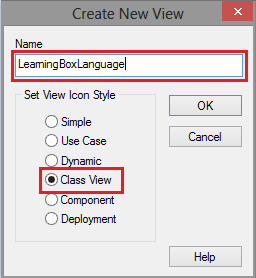
\includegraphics[width=0.33\textwidth]{ea_namePackage.png}
	\caption{Enter the name of the new package.}
	\label{fig:new_package_name}
\end{figure}
\FloatBarrier

\vspace{0.5cm}

\item[$\blacktriangleright$] Your \texttt{Project Browser} should now resemble Fig.~\ref{fig:new_package_completed}.

\begin{figure}[htbp]
	\centering
  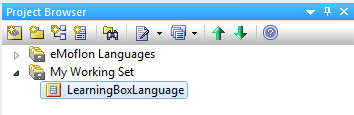
\includegraphics[width=0.5\textwidth]{ea_newPackage}
	\caption{State after creating the new package.}
	\label{fig:new_package_completed}
\end{figure}
\FloatBarrier

\clearpage
\item[$\blacktriangleright$] Now create a \texttt{New Diagram} (Fig.~\ref{fig:diagram}).

\begin{figure}[htbp]
	\centering
  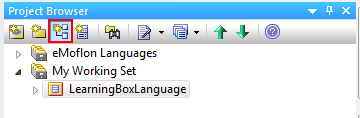
\includegraphics[width=0.5\textwidth]{ea_addDiagram}
	\caption{Add a diagram.}
	\label{fig:diagram}
\end{figure}
\FloatBarrier

\item[$\blacktriangleright$] In the dialogue that appears, (Fig.~\ref{fig:diagram_type}), choose \texttt{eMoflon Ecore Diagrams}, then select \texttt{OK}.

\begin{figure}[htbp]
	\centering
  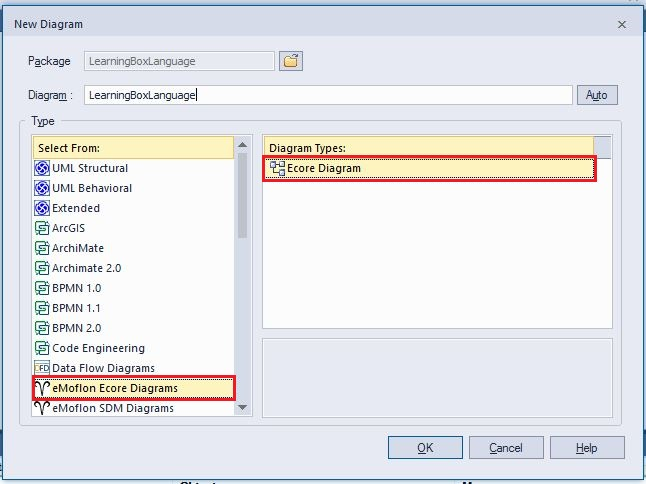
\includegraphics[width=0.8\textwidth]{ea_chooseDiagramType}
	\caption{Select the ecore diagram type}
	\label{fig:diagram_type}
\end{figure}
\FloatBarrier

 
\item[$\blacktriangleright$] After creating the new diagram, your  \texttt{Project Browser} should now resemble Fig.~\ref{fig:diagram_completed}.

\begin{figure}[htbp]
	\centering
  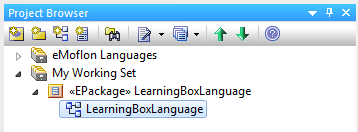
\includegraphics[width=0.5\textwidth]{ea_afterDiagramState}
	\caption{State after creating diagram}
	\label{fig:diagram_completed}
\end{figure}
\FloatBarrier

\item[$\blacktriangleright$] You have now just created the starting part for your Leitner's Box!

\fancyfoot[R]{$\triangleright$ \hyperlink{static:classes vis}{Next}}
\end{itemize}
